\chapter{Sprint 1 : socle sécurisé et administration}
\label{ch:sprint1}
\startcontents[chapters]
\chapterplan

\section{Introduction}

Le premier sprint pose les fondations de la plateforme. Avant de manipuler des données de paie, SEPAPaie doit savoir qui l'utilise, ce que chacun a le droit de faire et comment conserver la trace de ses actions. Planifié sur quatre semaines (tableau~\ref{tab:sprints}), il couvre la création et l'approbation des comptes, l'authentification, la gestion des sociétés débitrices, leur affectation aux Experts RH et le journal d'audit.

\section{Backlog du sprint}

Le backlog du sprint reprend les six premiers récits utilisateur du backlog produit (tableau~\ref{tab:backlog}). Le tableau~\ref{tab:backlog-s1} précise les tâches associées à chacun.

\begin{table}[H]
\centering
\footnotesize
\renewcommand{\arraystretch}{1.1}
\tablestyle
\begin{tabularx}{\textwidth}{|>{\centering\arraybackslash}p{0.9cm}|>{\raggedright\arraybackslash}p{5.2cm}|Y|}
\hline
\rowcolor{appMarine}\entete{N\textsuperscript{o}} & \entete{Récit utilisateur} & \entete{Principales tâches} \\
\hline
US1 & Créer un compte avec ma photo pour demander un accès & Formulaire d'inscription avec capture du visage ; contrôle d'unicité de l'identifiant et de l'adresse électronique ; calcul et conservation de l'empreinte du visage \\
\hline
US2 & M'authentifier par mot de passe et code à usage unique, ou par reconnaissance faciale & Vérification du mot de passe ; envoi, contrôle et expiration du code ; comparaison de visage ; émission du jeton de session \\
\hline
US3 & Valider les inscriptions et gérer les comptes et les rôles & Liste des demandes en attente ; approbation et rejet ; création directe d'un compte ; désactivation et réactivation \\
\hline
US4 & Gérer les sociétés débitrices et leurs coordonnées bancaires & Création et modification d'une société ; contrôle de l'IBAN et du BIC ; masquage de l'IBAN à l'affichage \\
\hline
US5 & Affecter les sociétés aux Experts RH & Affectation et retrait d'une société ; conservation de l'historique des affectations \\
\hline
US6 & Consulter le journal d'audit & Enregistrement des événements ; consultation réservée à l'administrateur, du plus récent au plus ancien \\
\hline
\end{tabularx}
\caption{Backlog du sprint 1}
\label{tab:backlog-s1}
\end{table}

\section{Conception}

\subsection{Diagramme de cas d'utilisation}

La figure~\ref{fig:uc-s1} détaille les cas d'utilisation de ce sprint. Deux acteurs système y apparaissent : le service Python, qui calcule et compare les empreintes de visage, et la messagerie, qui achemine le code à usage unique. L'administrateur gère les comptes, les sociétés et consulte le journal d'audit ; le Manager affecte les sociétés aux Experts RH ; tout utilisateur peut s'authentifier et gérer son propre visage de référence.

\begin{figure}[H]
\centering
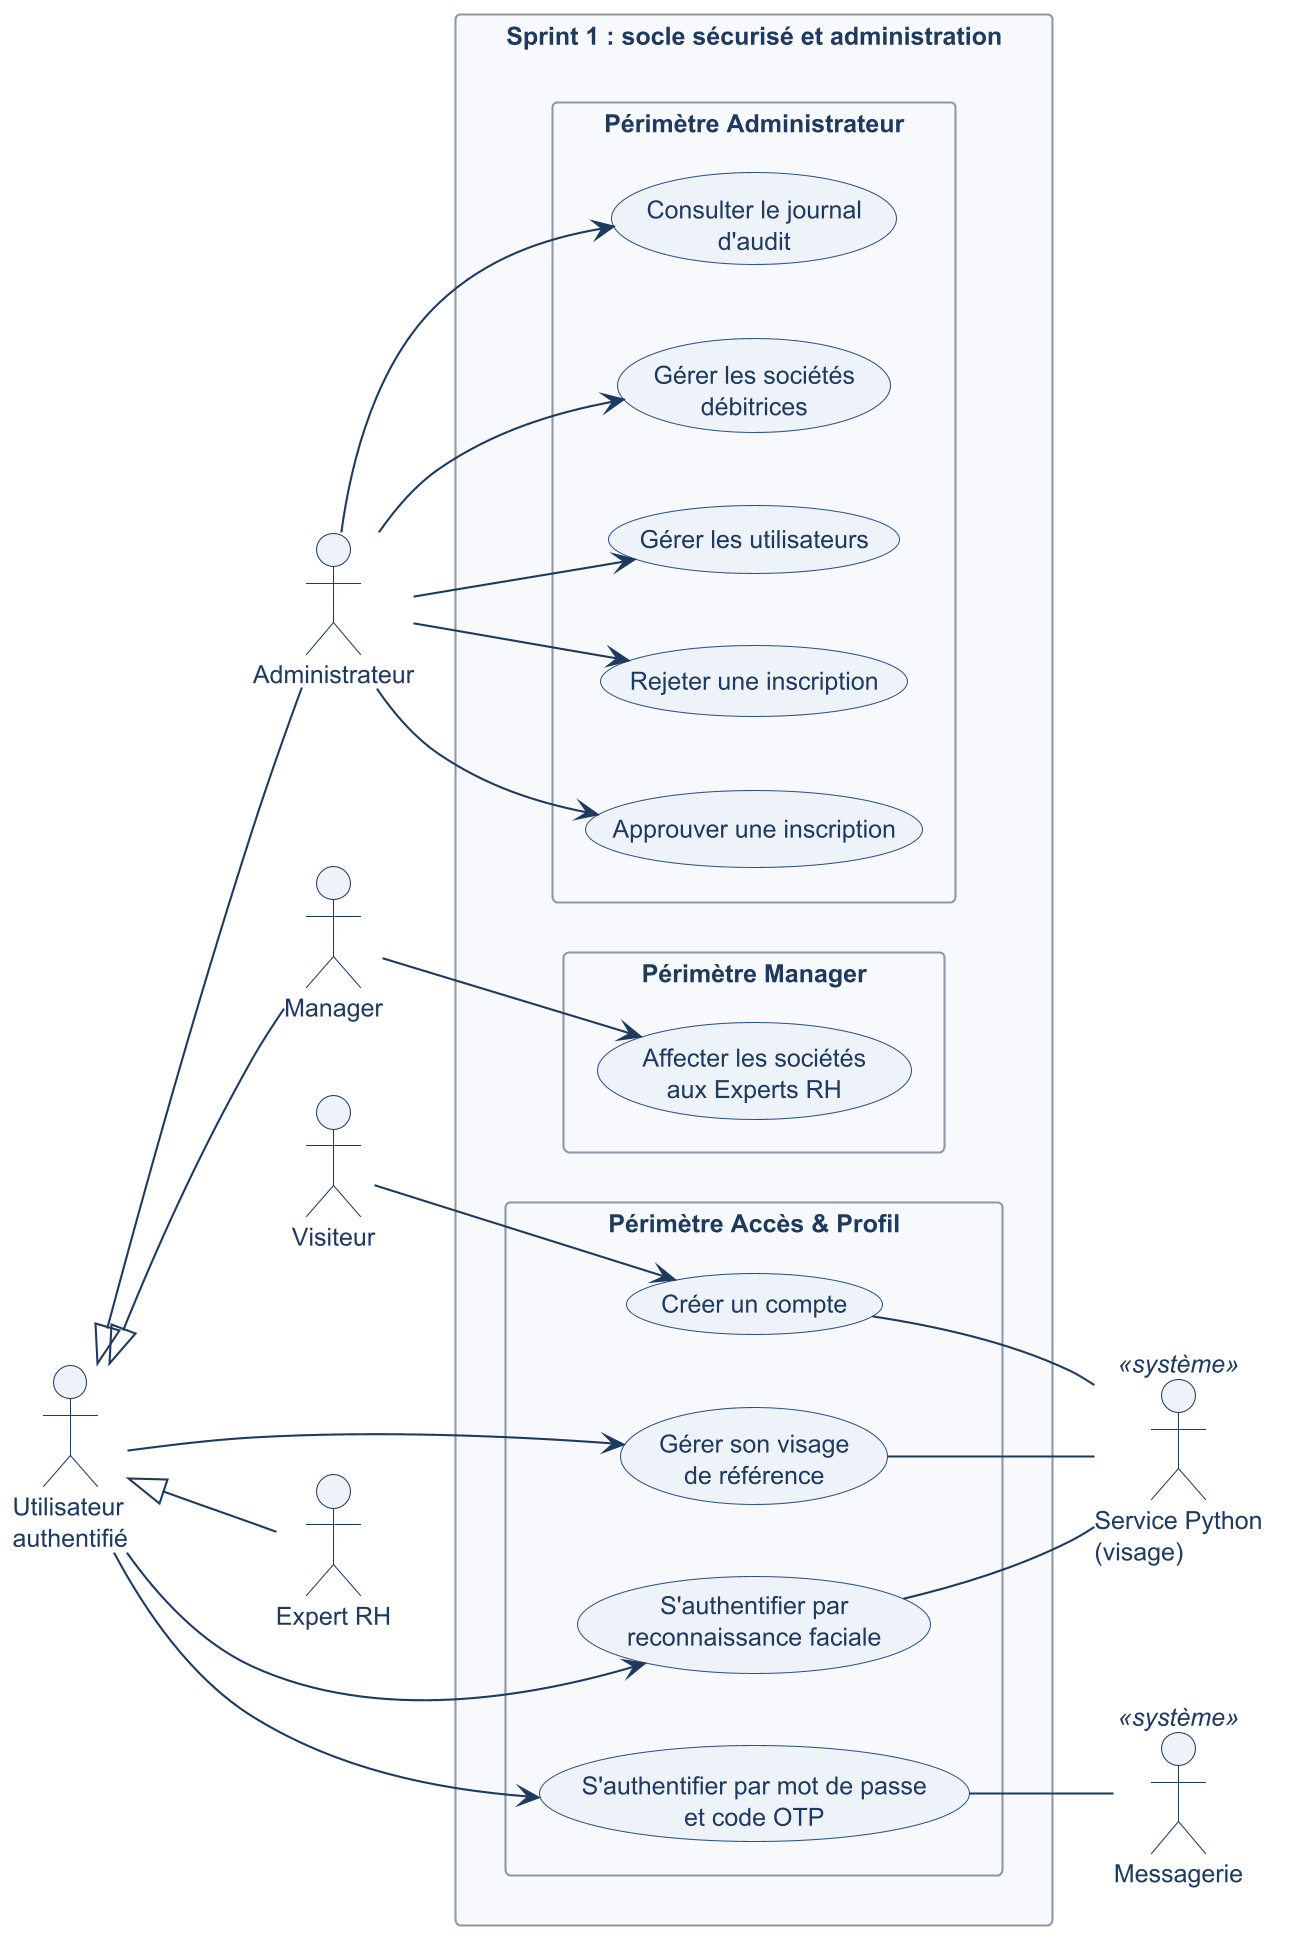
\includegraphics[height=0.38\textheight,width=\textwidth,keepaspectratio]{fig4_1_cas_utilisation_sprint1}
\caption{Cas d'utilisation du sprint 1}
\label{fig:uc-s1}
\end{figure}

\subsection{Inscription et approbation des comptes}

Un visiteur ne peut pas utiliser la plateforme dès son inscription. Il renseigne son identité, choisit le profil demandé et capture une photo de son visage. Le backend refuse la demande si l'identifiant ou l'adresse électronique existent déjà, ou si le profil n'est pas attribuable. Il sollicite ensuite le service Python pour obtenir l'empreinte numérique du visage. Seule cette empreinte est conservée en base ; la photo elle-même n'est pas enregistrée. Le compte est alors créé \textbf{inactif} et \textbf{non approuvé}, avec un mot de passe haché. La figure~\ref{fig:seq-inscription} illustre ce parcours.

\begin{figure}[H]
\centering
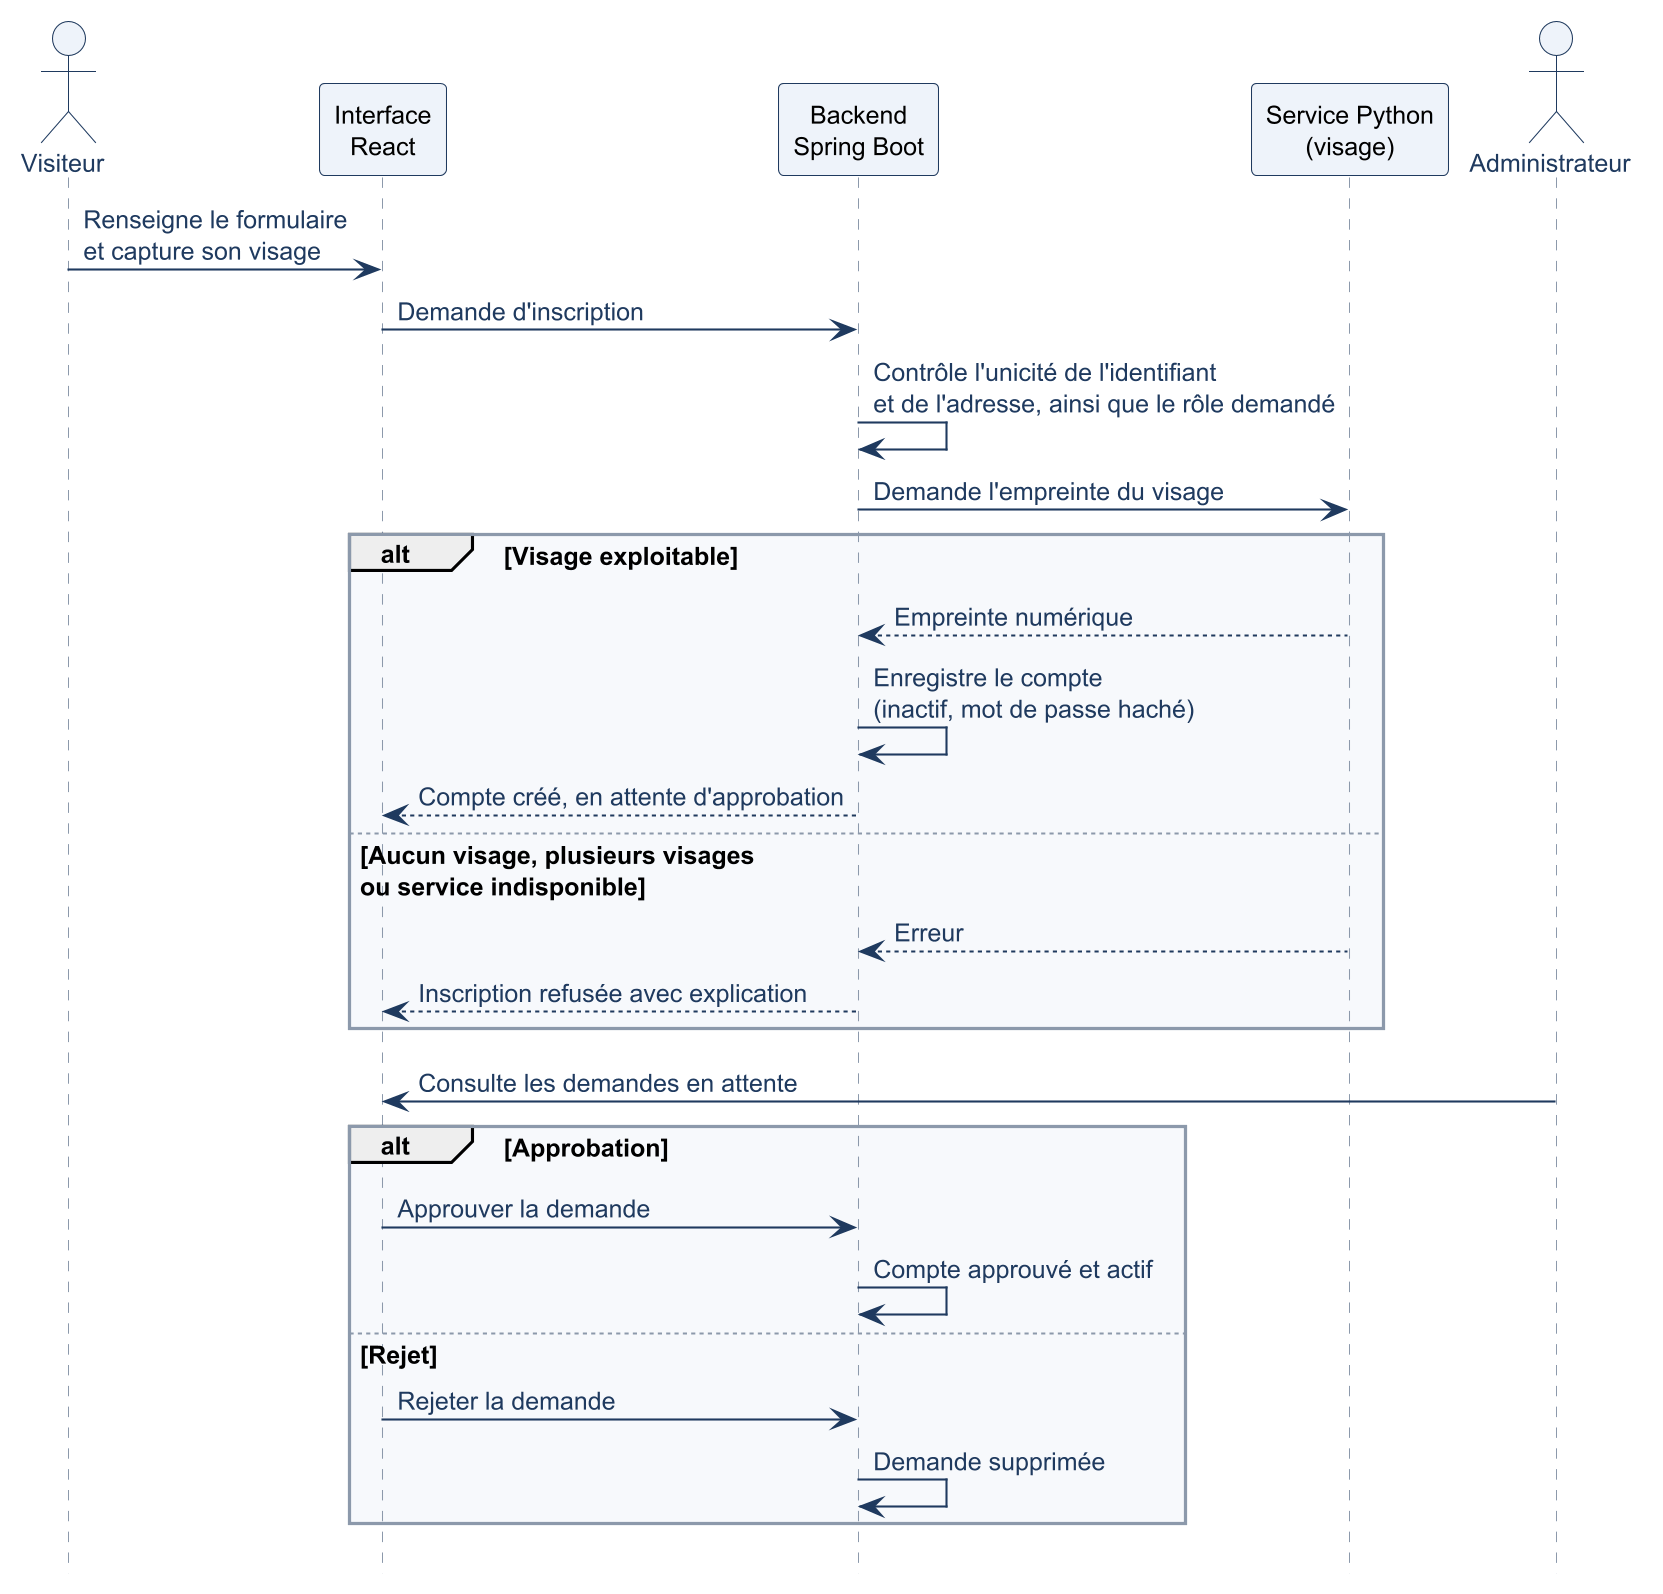
\includegraphics[height=0.55\textheight,width=\textwidth,keepaspectratio]{fig4_3_sequence_inscription}
\caption{Séquence d'inscription et d'approbation d'un compte}
\label{fig:seq-inscription}
\end{figure}

L'administrateur consulte les demandes en attente et les approuve ou les rejette telles qu'elles ont été formulées. L'approbation active le compte ; le rejet supprime la demande. L'administrateur peut aussi créer directement un compte, désactiver un compte existant ou le réactiver. La figure~\ref{fig:etats-compte} résume le cycle de vie d'un compte.

\begin{figure}[H]
\centering
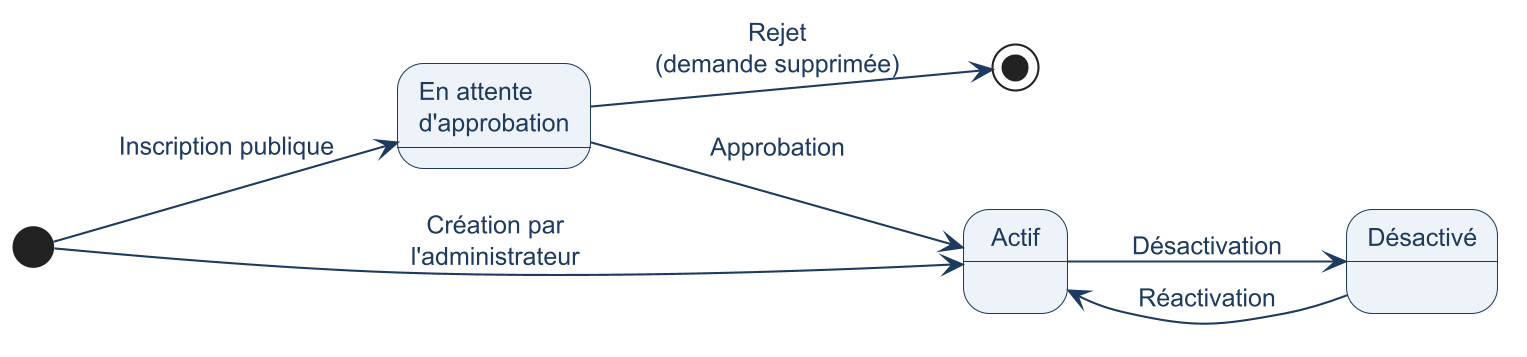
\includegraphics[width=\textwidth]{fig4_4_etats_compte}
\caption{Cycle de vie d'un compte utilisateur}
\label{fig:etats-compte}
\end{figure}

\subsection{Authentification adaptative}

SEPAPaie propose deux méthodes de connexion. Avec la première, l'utilisateur saisit son identifiant et son mot de passe, puis un code à usage unique envoyé par courriel. Avec la seconde, il présente son visage devant la caméra. La plateforme est dite \textbf{adaptative} parce que le backend, et non l'interface, décide si un second facteur est exigé : un mot de passe correct ne suffit jamais à ouvrir une session, alors qu'un visage reconnu constitue lui-même le facteur d'authentification. Cette règle est centralisée en un point unique du code, ce qui évite qu'une modification de l'interface ne la contourne.

La figure~\ref{fig:seq-auth} décrit la connexion par mot de passe. Le code est généré aléatoirement, conservé sous forme hachée et soumis à des limites décrites dans le tableau~\ref{tab:otp}.

\begin{figure}[H]
\centering
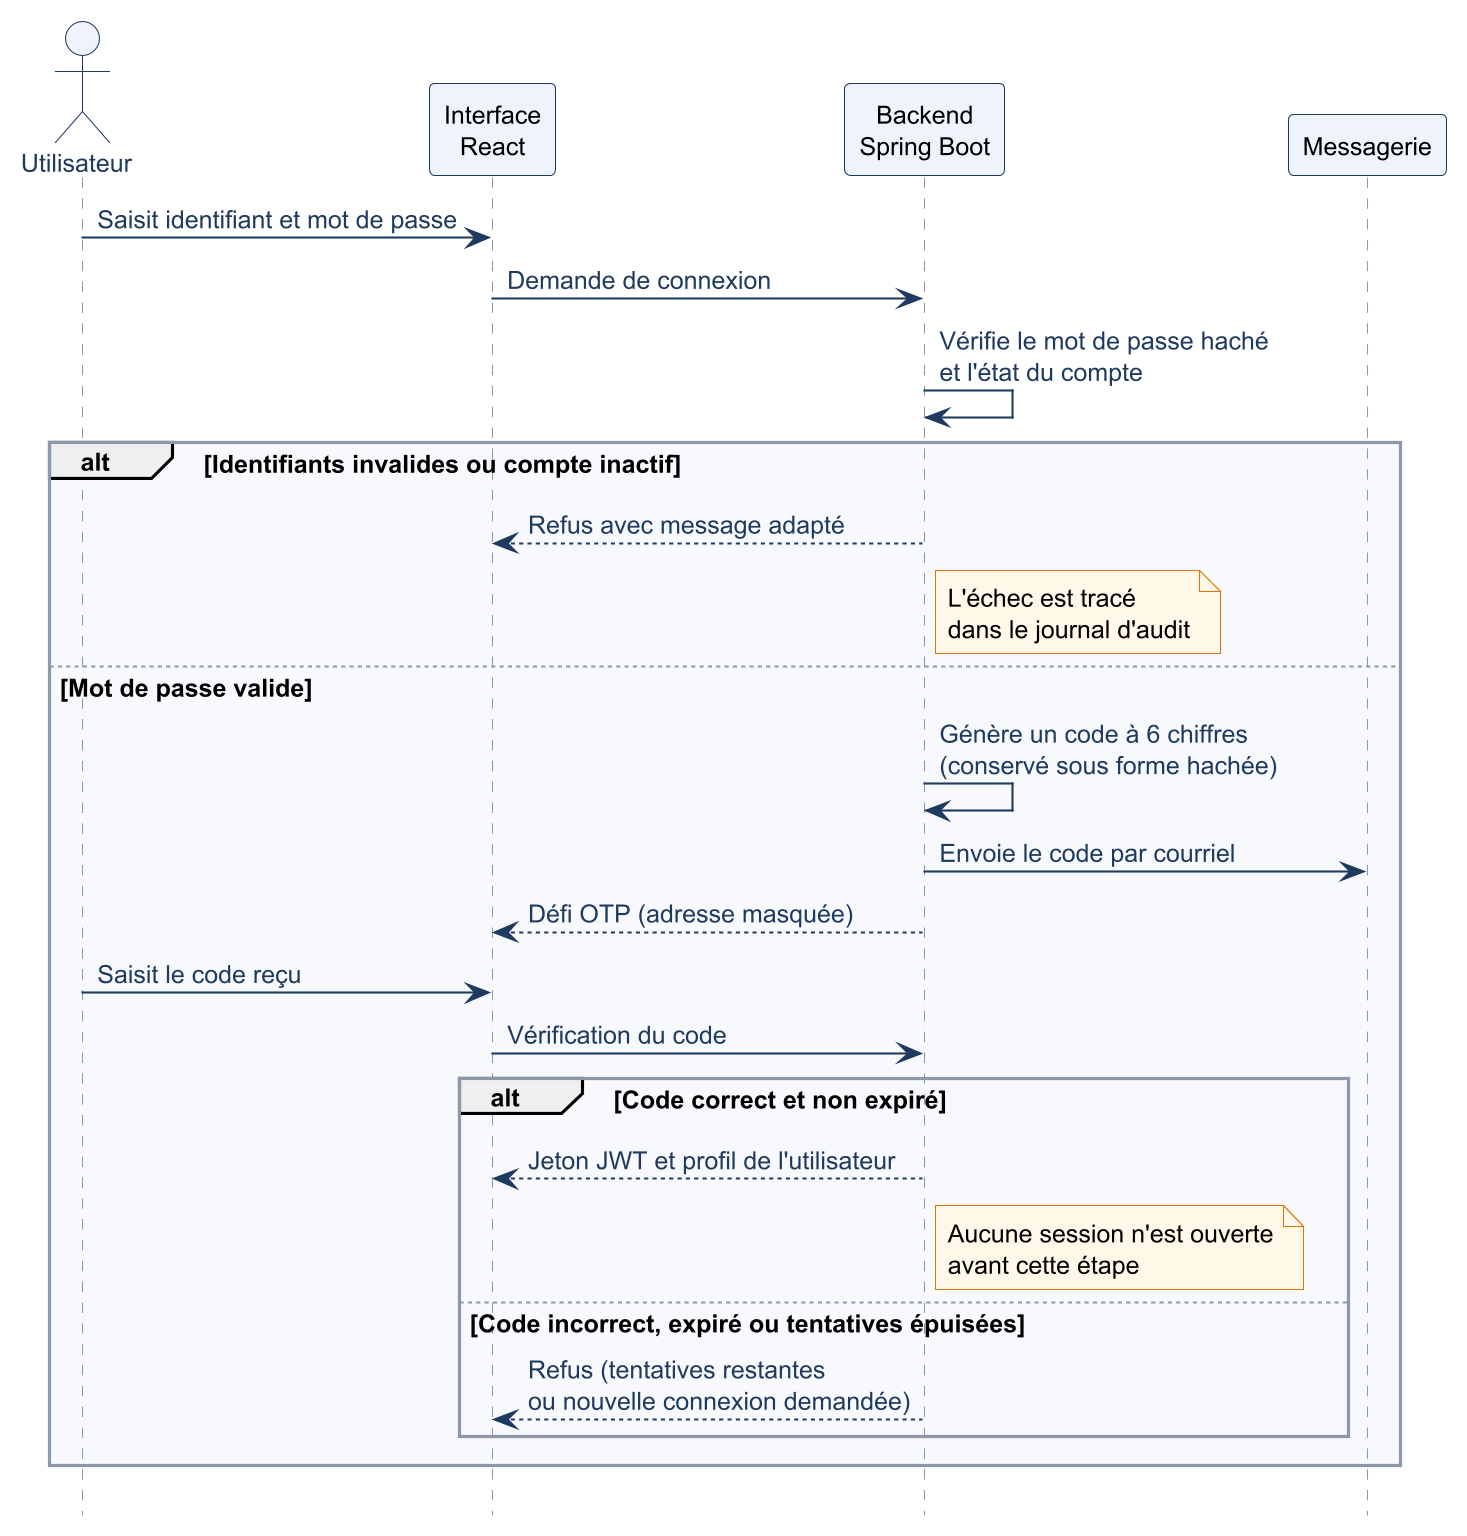
\includegraphics[height=0.58\textheight,width=\textwidth,keepaspectratio]{fig4_2_sequence_authentification}
\caption{Séquence d'authentification par mot de passe et code à usage unique}
\label{fig:seq-auth}
\end{figure}

\begin{table}[H]
\centering
\small
\renewcommand{\arraystretch}{1.25}
\tablestyle
\begin{tabularx}{\textwidth}{|>{\raggedright\arraybackslash}p{5cm}|Y|}
\hline
\rowcolor{appMarine}\entete{Paramètre} & \entete{Valeur par défaut} \\
\hline
Format du code & Six chiffres tirés par un générateur aléatoire cryptographique \\
\hline
Conservation du code & Sous forme hachée, jamais en clair \\
\hline
Durée de validité & Cinq minutes \\
\hline
Tentatives de saisie & Cinq au maximum ; au-delà, une nouvelle connexion est exigée \\
\hline
Renvois du code & Trois au maximum, avec un délai de trente secondes entre deux envois \\
\hline
\end{tabularx}
\caption{Paramètres du code à usage unique}
\label{tab:otp}
\end{table}

Ces valeurs sont configurables par variables d'environnement. Le principe retenu est de ne jamais accorder de session sur la seule foi d'un mot de passe : même si le réglage général du code à usage unique est désactivé, le parcours par mot de passe continue de l'exiger.

Pour la reconnaissance faciale, le backend transmet l'image capturée et l'empreinte de référence au service Python, qui détecte le visage, calcule son empreinte et mesure sa similarité avec la référence. Si elle dépasse le seuil recommandé par la bibliothèque, le visage est reconnu et le jeton est émis sans code. Dans tous les autres cas (visage refusé, service indisponible, erreur inattendue), aucun jeton n'est délivré et l'interface invite l'utilisateur à se connecter par mot de passe. L'indisponibilité du service Python ne peut donc jamais ouvrir un accès.

\subsection{Sécurité de la session et contrôle des droits}

Après une authentification réussie, le backend émet un jeton \textbf{JWT} signé, valable vingt-quatre heures. À chaque requête, un filtre en extrait l'identité, puis recharge l'utilisateur depuis la base : le rôle n'est donc pas lu dans le jeton, ce qui garantit que les droits appliqués sont ceux enregistrés au moment de l'appel. Aucune session n'est conservée côté serveur. Les mots de passe sont hachés avec l'algorithme BCrypt.

Les droits sont ensuite appliqués côté serveur. Les routes d'authentification sont publiques ; toutes les autres exigent un utilisateur authentifié. Chaque point d'accès est de plus protégé par une annotation qui reprend les expressions de droits centralisées dans une classe unique, conformément au tableau~\ref{tab:droits}. L'interface masque les menus non autorisés, mais cette présentation ne remplace pas le contrôle du serveur.

Le modèle de rôles a évolué en cours de projet : un premier découpage en quatre profils a été remplacé par les trois profils actuels (administrateur, Manager, Expert RH). Une migration exécutée au démarrage convertit les comptes existants vers les nouveaux rôles de façon idempotente et trace l'opération dans le journal d'audit. Les profils obsolètes ne sont plus attribuables.

\subsection{Gestion des utilisateurs}

La gestion des comptes est réservée à l'administrateur. Il y retrouve les demandes en attente, signalées par un message, ainsi que les comptes actifs et désactivés. Désactiver un compte empêche toute nouvelle connexion sans supprimer ses données, ce qui préserve l'historique des actions de la personne. Un utilisateur peut par ailleurs enregistrer, remplacer ou supprimer son visage de référence depuis son profil ; sans visage enregistré, seule la connexion par mot de passe lui est proposée.

\subsection{Sociétés débitrices}

Une société débitrice est caractérisée par un code, une raison sociale, un IBAN et un BIC. Lors de la création ou de la modification, l'IBAN est vérifié par le contrôle modulo~97 et le BIC par son format. Un enregistrement invalide est refusé avec un message explicite. Le code d'une société n'est pas modifiable, car il relie la société aux fiches de paie et aux fichiers générés. Une société n'est pas supprimée mais désactivée.

L'IBAN est masqué dans les listes : seuls les quatre premiers et les quatre derniers caractères apparaissent. Lors d'une modification, un champ IBAN laissé vide conserve la valeur existante, ce qui évite de réafficher la donnée complète. L'IBAN complet n'est communiqué qu'aux profils qui préparent les virements, puisque la génération du fichier en a besoin. Les coordonnées d'une société inconnue, inactive ou incomplète sont signalées comme telles afin d'expliquer pourquoi la préparation d'un fichier est impossible.

\subsection{Affectation des sociétés aux Experts RH}

Le Manager affecte chaque société à un Expert RH actif. Une société n'a qu'un expert à la fois, alors qu'un expert peut gérer plusieurs sociétés. Lorsqu'une société est réaffectée, l'affectation précédente est clôturée avec sa date de fin au lieu d'être écrasée : l'historique reste consultable et chaque changement est tracé dans le journal d'audit. Cette affectation définit le périmètre de travail de l'Expert RH, sur lequel s'appuient les contrôles d'accès par société présentés dans la suite du rapport.

\subsection{Journal d'audit}

Le journal enregistre, pour chaque événement, l'horodatage, l'utilisateur, le type d'action, un détail, l'adresse IP et le résultat. Dès ce sprint, il retient les étapes de connexion (code envoyé, connexion réussie, échec), les migrations de rôles et les changements d'affectation. Il est enrichi aux sprints suivants par les opérations sur les fiches et les fichiers. Seul l'administrateur peut le consulter. L'interface affiche les cent événements les plus récents, du plus récent au plus ancien, à partir d'une interface de programmation qui accepte la pagination, et aucune fonction ne permet d'en modifier le contenu. L'enregistrement des événements reste en revanche commun à tous les profils.

\subsection{Interfaces réalisées}

Les écrans suivants proviennent de l'application exécutée localement avec des comptes de démonstration. La figure~\ref{fig:ecrans-connexion} présente la connexion, dans laquelle le choix entre mot de passe et reconnaissance faciale est proposé sur le même écran, puis l'étape de saisie du code reçu. L'adresse de destination y est masquée.

\begin{figure}[H]
\centering
\begin{subfigure}[t]{0.36\textwidth}
\centering
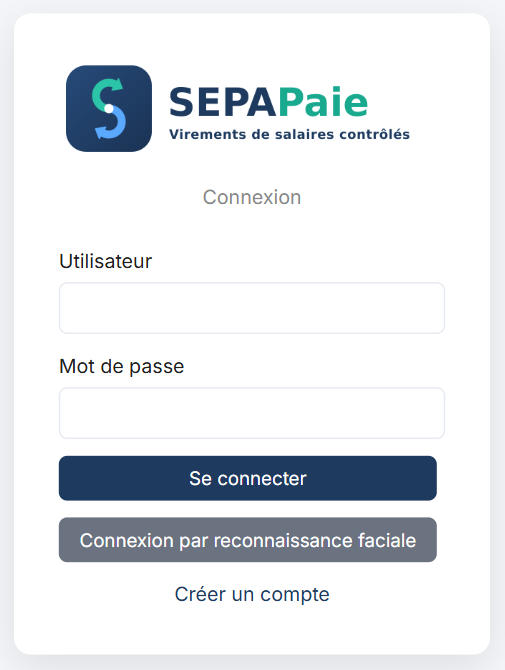
\includegraphics[width=\textwidth]{fig4_login}
\caption{Saisie des identifiants}
\end{subfigure}
\hspace{0.05\textwidth}
\begin{subfigure}[t]{0.36\textwidth}
\centering
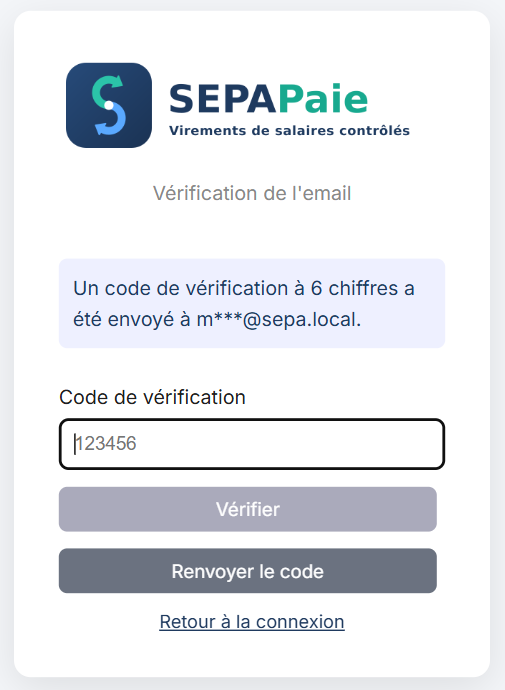
\includegraphics[width=\textwidth]{fig4_otp}
\caption{Saisie du code reçu}
\end{subfigure}
\caption{Écrans de connexion}
\label{fig:ecrans-connexion}
\end{figure}

La figure~\ref{fig:ecran-societes} présente la liste des sociétés débitrices, dont l'IBAN est masqué, et la figure~\ref{fig:ecran-audit} le journal d'audit, où chaque connexion laisse la trace de l'envoi du code puis de sa vérification.

\begin{figure}[H]
\centering
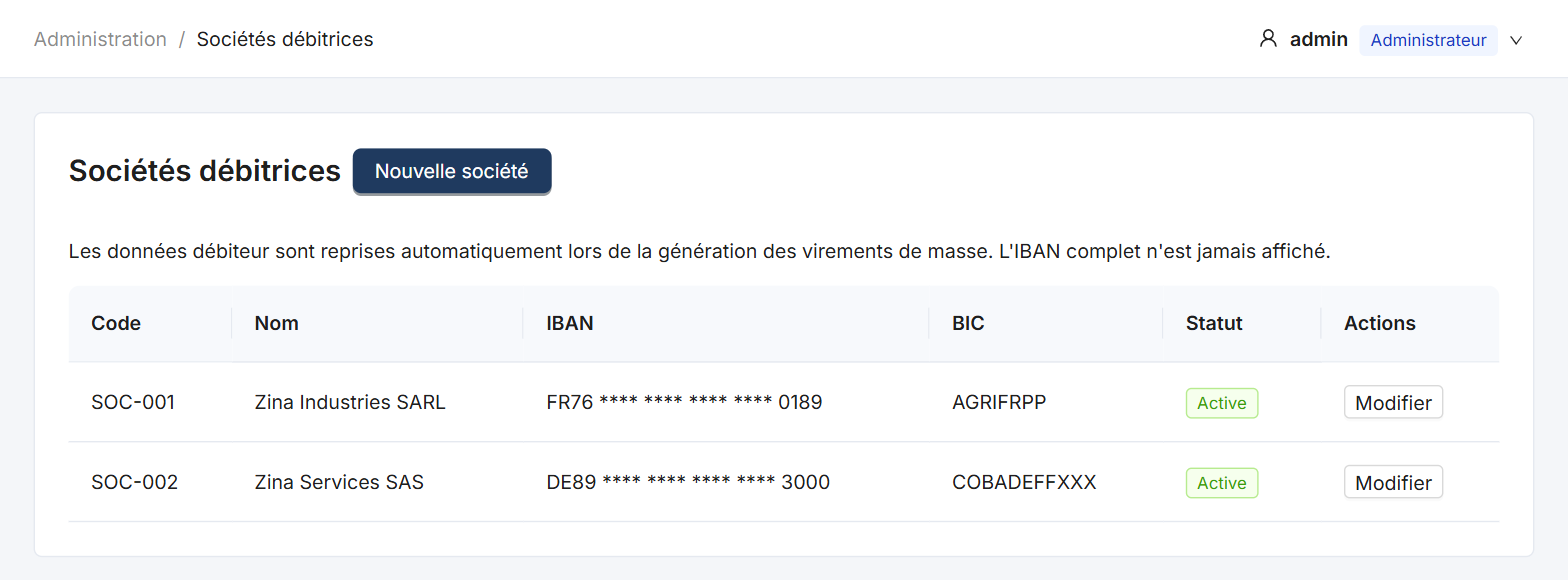
\includegraphics[width=0.9\textwidth]{fig4_societes}
\caption{Sociétés débitrices (profil administrateur)}
\label{fig:ecran-societes}
\end{figure}

\begin{figure}[H]
\centering
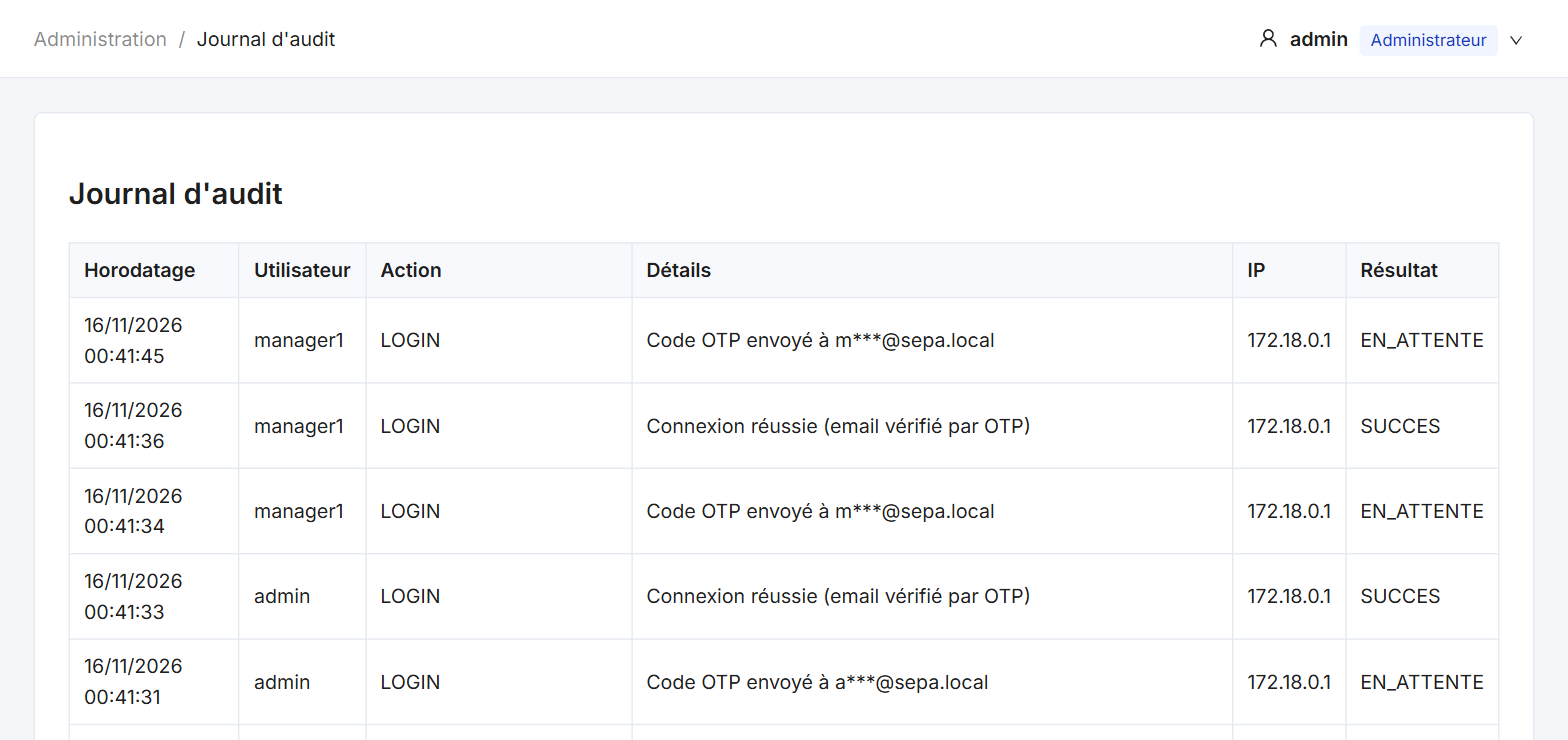
\includegraphics[width=0.9\textwidth]{fig4_audit}
\caption{Journal d'audit (profil administrateur)}
\label{fig:ecran-audit}
\end{figure}

\section{Conclusion}

Le sprint 1 a livré le socle des suivants : comptes soumis à approbation, authentification qui n'accorde jamais d'accès sur la seule foi d'un mot de passe, droits appliqués côté serveur, sociétés débitrices contrôlées, affectations historisées et journal d'audit. Le chapitre suivant présente le sprint 2, consacré aux données de paie, aux schémas XSD et à la génération du fichier SEPA.

